% Author: Izaak Neutelings (Februari, 2020)
% page 8 https://archive.org/details/StaticAndDynamicElectricity
% https://tex.stackexchange.com/questions/56353/extract-x-y-coordinate-of-an-arbitrary-point-on-curve-in-tikz
% https://tex.stackexchange.com/questions/412899/tikz-calculate-and-store-the-euclidian-distance-between-two-coordinates

\documentclass[border=3pt,tikz]{standalone}
\usepackage{amsmath} % for \dfrac
\usepackage{physics}
\usepackage{tikz,pgfplots}
\usetikzlibrary{angles,quotes} % for pic (angle labels)
\usetikzlibrary{decorations.markings}
\tikzset{>=latex} % for LaTeX arrow head

\usepackage{xcolor}
\colorlet{Ecol}{orange!90!black}
\colorlet{veccol}{green!45!black}
\tikzstyle{EField}=[thick,Ecol]
\def\xmax{5.0}
\def\ymax{3.3}
\def\tick#1#2{\draw[thick] (#1) ++ (#2:0.03*\ymax) --++ (#2-180:0.06*\ymax)}


\begin{document}


% ELECTRIC FIELD of a CHARGED SPHERE
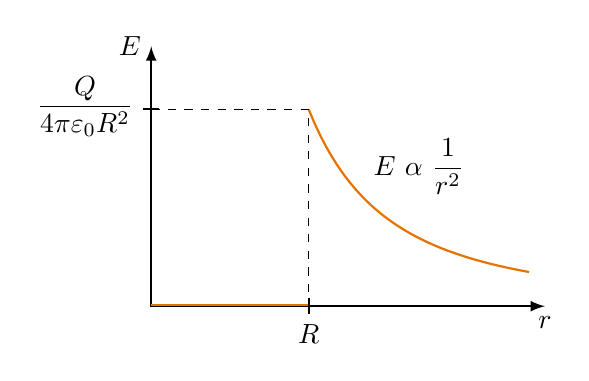
\begin{tikzpicture}

    \def\kQ{10}
    \def\R{2.0}
    \coordinate (O) at (0,0);
    \coordinate (X) at (\xmax,0);
    \coordinate (Y) at (0,\ymax);
    \coordinate (P) at (\R,\kQ/\R^2);
    \coordinate (Px) at (\R,0);
    \coordinate (Py) at (0,\kQ/\R^2);

    % AXIS
    \draw[<->,thick]
    (X) node[below] {$r$} -- (O) -- (Y) node[left] {$E$};
    \tick{Py}{ 0} node[below=-1,left] {$\dfrac{Q}{4 \pi \varepsilon_0 R^2}$};
    \tick{Px}{90} node[below] {$R$};

    % PLOT
    \draw[EField,samples=100,smooth,variable=\x,domain=\R:0.96*\xmax]
    plot(\x,\kQ/\x^2);
    \draw[EField]
    (0,0.004*\ymax) --++ (Px);
    \node[above right] at (2.7,1.3) {$E\ \alpha\ \dfrac{1}{r^2}$};
    \draw[dashed]
    (Py) -- (P) -- (Px);

\end{tikzpicture}
\end{document}